У цьому розіділі наведено числові результати та їх аналіз для задач,
які розв'язано у попередніх розділах.
Усі подальщі розрахунки проведено для для сталі ($E=200$ ГПА, $\mu=0.25$) та зафіксовані розміри прямокутника по осі $y$, $0 \le y \le 15$.
В подальшому для того, щоби розглянути залежності від геометрії тіла,
розмір області буде змінюватись по осі $x$.

\subsection{Статичні задачі}

У цьому пункті проаналізовано статичні задачі теорії пружності для прямокутної області за різних умов на бічних гранях.
Спочатку розлянемо випадок задачі за умов ідеального контакту на бічних гранях
розв'зок якої наведено у Підрозділі 3.1.
\begin{figure}[h!]
    \begin{center}
        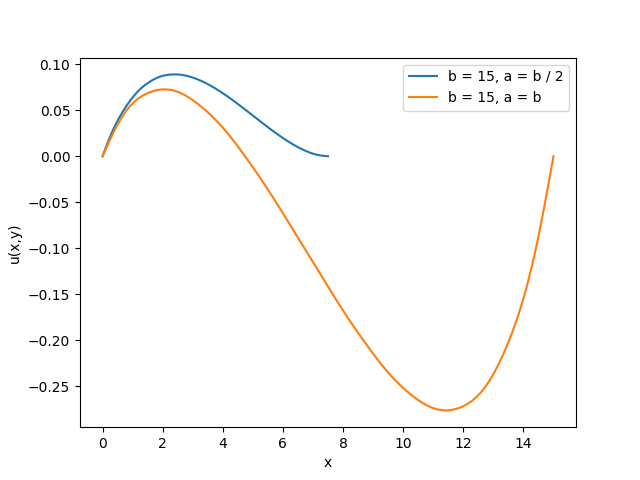
\includegraphics[width=0.49\textwidth, scale=1]{images/results/static_1/u(x,b)1.png}
        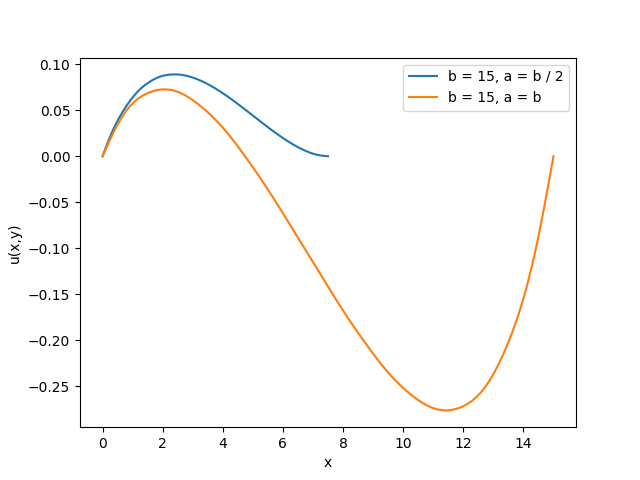
\includegraphics[width=0.49\textwidth, scale=1]{images/results/static_1/u(x,b)2.png}
        \caption{Переміщення $u(x, b)$}\label{static_1_u(x,b)1}
    \end{center}
\end{figure}

На Рис \ref{static_1_u(x,b)1} зображено функція переміщеня $u(x, y)$ при $y=b$.
З графіків видно виконання граничних умов на бічних гранях $u(x,y) |_{x=0} = 0$, $u(x,y) |_{x=a} = 0$,
що підтверджує коректність знайденого розв'язку.
Також можна побачити, що при різних розмірах прямокутної області міняється максимальне та мінальне значення функції пермешінення,
при $a = 2b$ мінімум функції набуває найменьшого значення, а для випадку $a = b / 2$ максимум функції набуває найбільшого значення.


\subsubsection{Випадок граничних умов другої основної задачі теорії пружності на бічних гранях}



\subsection{Динамічні задачі}